\documentclass{beamer}
\usepackage[latin1]{inputenc}
\usepackage{graphicx}
\usepackage{listings}
\usepackage{color}
\usepackage{array}

\usepackage{color}
\definecolor{dkgreen}{rgb}{0,0.6,0}
\definecolor{gray}{rgb}{0.5,0.5,0.5}
\definecolor{mauve}{rgb}{0.58,0,0.82}
\lstset{
language=[x86masm]Assembler,
alsolanguage=C,
basicstyle=\scriptsize, 
numbers=left, 
numberstyle=\tiny\color{gray}, 
showspaces=false, 
showstringspaces=false, 
keywordstyle=\color{blue},
commentstyle=\color{dkgreen},
stringstyle=\color{mauve},
}

\usetheme{Berlin}
\usecolortheme{beaver}
\title[Baggy Bounds with LLVM]{6.858 Final Project: Baggy Bounds with LLVM}

\author{Anton Anastasov \and
Chirantan Ekbote \and
  Travis Hance
}

\date{December 11, 2013}

\begin{document}
\frame{\titlepage}

%slide
\begin{frame}{Plan: Write transformation pass on LLVM Intermediate Representation (IR) to implement baggy bounds pointer arithmetic}
\begin{enumerate}
\item Align every global and stack allocation to correct boundary.
\item On stack allocation, update \texttt{size\_lookup\_table}, marking a region with its allocation size.
\item Augment pointer arithmetic with baggy bounds checks.
\item Implement binary buddy allocator for dynamic allocations.
\end{enumerate}
\end{frame}
%slide
\begin{frame}{Results}
\begin{figure}[p]
\centering
\graphicspath{ {../test/} }
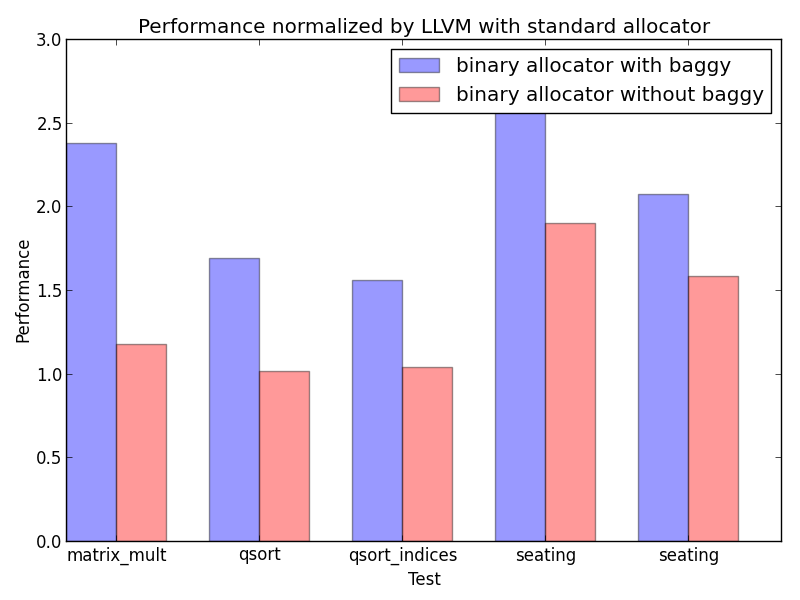
\includegraphics[scale=0.45]{figure_1.png}
\end{figure}
\end{frame}

\begin{frame}{Q \& A}

{\LARGE Thank you. Questions?}
\end{frame}
\end{document}
